
\documentclass[a4paper,12pt]{article}

\usepackage[utf8]{inputenc}
\usepackage[margin=1in]{geometry}
\usepackage{xcolor}
\usepackage{graphicx}
\usepackage{wrapfig}
\usepackage[skip=10pt plus1pt, indent=40pt]{parskip}
\usepackage{hyperref}
\usepackage{afterpage}
\author{\large{Rinik C S}}
\title{\textcolor{blue}{\huge{Plant Pathology}}}
\begin{document}
\pagecolor{yellow}\afterpage{\nopagecolor}
\maketitle
\newpage



\tableofcontents

\newpage
\section{Aim}
To gain a comprehensive understanding of common plant diseases, their causative agents, and effective control strategies, contributing to the knowledge base in plant pathology and agricultural science.
\section{Introduction}
 \subsection{Pathology}
 Pathology, medical specialty concerned with the determining causes of disease and the structural and functional changes occurring in abnormal conditions.
\subsection{Plant Pathology}
Plant pathology or plant disease, an impairment of the normal state of a plant that interrupts or modifies its vital functions.\\
\begin{wrapfigure}{l}{2in}
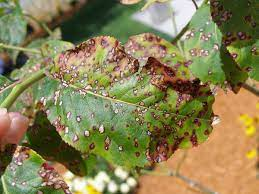
\includegraphics[scale=0.5]{leaf}
\caption{Leaf spot diseases of trees and shrubs}
\end{wrapfigure}
 All species of plants, wild and cultivated alike, are subject to disease. Although each species is susceptible to characteristic diseases, these are, in each case, relatively few in number. The occurrence and prevalence of plant diseases vary from season to season, depending on the presence of the pathogen, environmental conditions, and the crops and varieties grown. Some plant varieties are particularly subject to outbreaks of diseases while others are more resistant to them.
 
 
 
 
 
\subsection{Nature and importance of plant diseases(optional)}
Plant diseases are known from times preceding the earliest writings. Fossil evidence indicates that plants were affected by disease 250 million years ago. The Bible and other early writings mention diseases, such as rusts, mildews, and blights, that have caused famine and other drastic changes in the economy of nations since the dawn of recorded history. Other plant disease outbreaks with similar far-reaching effects in more recent times include late blight of potato in Ireland (1845$-$60); powdery and downy mildews of grape in France (1851 and 1878); coffee rust in Ceylon (now Sri Lanka; starting in the 1870s); Fusarium wilts of cotton and flax; southern bacterial wilt of tobacco (early 1900s); Sigatoka leaf spot and Panama disease of banana in Central America (1900$-$65); black stem rust of wheat (1916, 1935, 1953$-$54); southern corn leaf blight (1970) in the United States; Panama disease of banana in Asia, Australia, and Africa (1990 to present); and coffee rust in Central and South America (1960, 2012 to present). Such losses from plant diseases can have a significant economic impact, causing a reduction in income for crop producers and distributors and higher prices for consumers.

Loss of crops from plant diseases may also result in hunger and starvation, especially in less-developed countries where access to disease-control methods is limited and annual losses of 30 to 50 percent are not uncommon for major crops. In some years, losses are much greater, producing catastrophic results for those who depend on the crop for food. Major disease outbreaks among food crops have led to famines and mass migrations throughout history. The devastating outbreak of late blight of potato (caused by the water mold Phytophthora infestans) that began in Europe in 1845 brought about the Great Famine that caused starvation, death, and mass migration of the Irish. Of Ireland’s population of more than eight million, approximately one million (about 12.5 percent) died of starvation or famine-related illness, and 1.5 million (almost 19 percent) emigrated, mostly to the United States, as refugees from the destructive blight. This water mold thus had a tremendous influence on economic, political, and cultural development in Europe and the United States. During World War I, late blight damage to the potato crop in Germany may have helped end the war.
\subsection{Diseases a normal part of nature}
Plant diseases are a normal part of nature and one of many ecological factors that help keep the hundreds of thousands of living plants and animals in balance with one another. Plant cells contain special signaling pathways that enhance their defenses against insects, animals, and pathogens. One such example involves a plant hormone called jasmonate (jasmonic acid). In the absence of harmful stimuli, jasmonate binds to special proteins, called JAZ proteins, to regulate plant growth, pollen production, and other processes. In the presence of harmful stimuli, however, jasmonate switches its signaling pathways, shifting instead to directing processes involved in boosting plant defense. Genes that produce jasmonate and JAZ proteins represent potential targets for genetic engineering to produce plant varieties with increased resistance to disease.
 
Humans have carefully selected and cultivated plants for food, medicine, clothing, shelter, fibre, and beauty for thousands of years. Disease is just one of many hazards that must be considered when plants are taken out of their natural environment and grown in pure stands under what are often abnormal conditions.

Many valuable crop and ornamental plants are very susceptible to disease and would have difficulty surviving in nature without human intervention. Cultivated plants are often more susceptible to disease than are their wild relatives. This is because large numbers of the same species or variety, having a uniform genetic background, are grown close together, sometimes over many thousands of square kilometres. A pathogen may spread rapidly under these conditions.

\subsection{Plant disease}

The study of plant diseases is called plant pathology. Pathology is derived from the two Greek words pathos (suffering, disease) and logos (discourse, study). Plant pathology thus means a study of plant diseases.

In general, a plant becomes diseased when it is continuously disturbed by some causal agent that results in an abnormal physiological process that disrupts the plant’s normal structure, growth, function, or other activities. This interference with one or more of a plant’s essential physiological or biochemical systems elicits characteristic pathological conditions or symptoms.

Plant diseases can be broadly classified according to the nature of their primary causal agent, either infectious or noninfectious. Infectious plant diseases are caused by a pathogenic organism such as a fungus, bacterium, mycoplasma, virus, viroid, nematode, or parasitic flowering plant. An infectious agent is capable of reproducing within or on its host and spreading from one susceptible host to another. Noninfectious plant diseases are caused by unfavourable growing conditions, including extremes of temperature, disadvantageous relationships between moisture and oxygen, toxic substances in the soil or atmosphere, and an excess or deficiency of an essential mineral. Because noninfectious causal agents are not organisms capable of reproducing within a host, they are not transmissible.

Noninfectious plant diseases are caused by unfavourable growing conditions, including extremes of temperature, disadvantageous relationships between moisture and oxygen, toxic substances in the soil or atmosphere, and an excess or deficiency of an essential mineral. Because noninfectious causal agents are not organisms capable of reproducing within a host, they are not transmissible.

In nature, plants may be affected by more than one disease-causing agent at a time. A plant that must contend with a nutrient deficiency or an imbalance between soil moisture and oxygen is often more susceptible to infection by a pathogen, and a plant infected by one pathogen is often prone to invasion by secondary pathogens. The combination of all disease-causing agents that affect a plant make up the disease complex. Knowledge of normal growth habits, varietal characteristics, and normal variability of plants within a species$-$as these relate to the conditions under which the plants are growing$-$is required for a disease to be recognized.


\section{Disease development and transmission}
\subsection{Pathogenesis and saprogenesis}
Pathogenesis is the stage of disease in which the pathogen is in intimate association with living host tissue. \\ Three fairly distinct stages are involved:
\begin{description}
\item Inoculation: transfer of the pathogen to the infection court, or area in which invasion of the plant occurs.
\item Incubation: the period of time between the arrival of the pathogen in the infection court and the appearance of symptoms.
\item Infection: the appearance of disease symptoms accompanied by the establishment and spread of the pathogen.
\end{description}
One of the important characteristics of pathogenic organisms, in terms of their ability to infect, is virulence.










\end{document}
